\section{Automatic and Human Evaluation}\label{sec:eval}


To properly evaluate our models we relied on a combination of existing and novel metrics which are compiled in the newly proposed concept of metric card \Cref{metriccard}. In this section, we specifically detailed the novel contributions in automatic expressivity metrics, followed by presenting results of our models in terms of robustness and several human evaluation protocols.

\subsection{Automatic Expressivity Metrics}

\label{sec:expressivity_metrics}
To ensure the quality of \seamlessexpressive, we relied on measures that evaluate the prosodic consistency of source and target speech.


Early work on comparing prosody across languages \citep{cummins:prosody} used an LSTM-based (\cite{hochreiter:lstm}) model with features based on $F_0$ contour and amplitude envelope.
In \cite{ward2023dral,avila2023prosody}, the authors created an English-Spanish corpus (DRAL) and provided an analysis of the prosodic relation between a pair of audios by calculating the Spearman correlation of 100 features (e.g., intensity, speaking rate, pitch) and provided a simple metric corresponding to the Euclidean distance between the two prosodic representations.

We contribute two types of automatic measures of prosodic preservation in speech translation: 1) \comparator to evaluate prosody at the sentence level and 2) a rhythm evaluation toolkit.

\paragraph{\comparator.}  
\label{sec:comparator}
Our main measure of prosodic preservation, PCP (\citet{huang2023holistic}; see also \Cref{sec:pcp}), corresponds to human judgments (using a 4-point Likert scale) of how similarly two spoken utterances sound in prosody. \comparator is a neural model trained to predict PCP scores of ``sentence-level prosody similarity''. This model has an architecture similar to BLASER \citep{chen-etal-2023-blaser}: embedding vectors of two audios (in our case, obtained by pooling embeddings from the 9th layer of an XLS-R model \citep{conneau2020unsupervised}) are passed into a small fully-connected neural network that predicts the target score. 

We trained \comparator with two tasks: supervised regression and an unsupervised contrastive task. For regression, we annotated with simplified PCP in which annotators are asked about a single expressive dimension ``Overall Manner,'' analogous to the dimension ``Overall Expressive Intent`` described in \Cref{sec:humaneval_protocols}. In total, we collected nearly 800 sentence pairs for each translation direction (from French, Italian, German, Mandarin, and Spanish to English). %
To ensure that the dataset contains audio pairs with diverse prosodic similarity degrees, we compiled it from several sources:
\begin{itemize}[noitemsep,nolistsep]
    \item Audio pairs from multilingual videos (\Cref{sec:dubbed_data}), with naturally diverse quality;
    \item M4T training data (\Cref{sec:offline:data}), with either original or re-synthesized target speech;
    \item Audio pairs synthesized using cTTS, with both matching and mismatching speech rate and pauses (following \Cref{ctts_aug});
    \item mExpresso audio pairs (\Cref{subsec:mexpresso}) with matching and mismatching styles.
\end{itemize}

As a source of contrastive data, we used the parallel corpus from multilingual videos (\Cref{sec:dubbed_data}); the model is trained to predict higher scores for positive examples (the original audio pairs) than for hard negative examples (re-combined audio pairs with similar semantic embeddings of their transcriptions). 
We return to the discussion of human- and automatic-metric correlation under our human evaluation test sets in \Cref{sec:human_eval_correlation_analysis}.

We evaluated the resulting model with three metrics on a test set annotated with PCP: item-level and system-level Spearman correlations and RMSE. As \Cref{tab:eval:comparator-correlation} shows, the model performs robustly across languages, and its results are comparable to human-level, computed as judgments of a single randomly chosen annotator compared to the median score of the other annotators. We also validate the model by comparing it to a simple baseline: cosine similarity of the same XLS-R speech embeddings, rescaled to minimize RMSE on the test set. The \comparator model demonstrates much better item- and system-level correlation with the target than the baseline.

The model card for \comparator is given in \Cref{app:comparator_model_card}.


\begin{table}[ht!]
    \centering
    \small
    \begin{tabular}{lcccccccc}
        \toprule
         & \multicolumn{6}{c}{\textbf{\comparator}} & \textbf{baseline}& \textbf{human} \\\cmidrule(r){2-7}\cmidrule(l){8-8} \cmidrule(l){9-9}
        \textbf{System} & deu & spa & fra & ita & cmn & \textbf{avg} &\textbf{avg} & \textbf{avg}  \\ 
        \midrule
        Item-level correlation $\uparrow$ & 0.58 & 0.50 & 0.44 & 0.50 & 0.44 & 0.49 & 0.31 & 0.46 \\
        System-level correlation $\uparrow$ & 0.60 & 0.58 & 0.60 & 0.77 & 0.72 & 0.65 & 0.28 & 0.84 \\
        RMSE $\downarrow$ & 0.68 & 0.61 & 0.88 & 0.85 & 0.90 & 0.79 & 0.81 & 0.97 \\
        \bottomrule
    \end{tabular}
\caption{\textbf{Evaluation of the \comparator model.} To estimate human-level performance, for each sample, we randomly selected the label from one randomly chosen annotator and compared it to the median label from the other annotators. The same target is used to estimate model performance. By ``system'' here, we denote a combination of the data source and the method to obtain the target audio. 
}
\label{tab:eval:comparator-correlation}
\end{table}

\paragraph{Rhythm evaluation toolkit.}
\label{sec:local-prosody-tools}
To complement \comparator, a blackbox predictor of overall prosodic similarity, we designed tools for quantifying and comparing several individual aspects of prosody in a more interpretable way. More specifically, we focused on evaluating rhythm as realized in speech rate and pauses.
\begin{itemize}[noitemsep,nolistsep]
    \item \textbf{Speech rate}: the number of syllables per second\footnote{Despite syllable-level speech rate showing lower correlation with human judgments on Spanish-English data than with other units of content, we chose this unit based on linguistic considerations—as the most generalizable across diverse languages.}. We obtained the syllables by running the ``syllables'' python package on the transcription (except for Mandarin, where we counted each character as a syllable) and dividing their number by the net duration of the audio in seconds, computed using Silero VAD \citep{SileroVAD}.
    \item \textbf{Pauses}: we detected pauses and their durations with Silero VAD and located them between the words of the transcription using the \unitytwo aligner (\Cref{sec:offline:unity2:unsup_aligner}). To evaluate whether a pause is located correctly in the translation, we aligned the source and translation words with AwesomeAlign \citep{dou2021awesomealign}, and used the proportion of word alignment edges that \textit{do not cross} the edge connecting two matched pauses as the metric of pause location. For each source-translation pair, we computed the joint score as the average product of the location score of each pause and its shorter-to-longer duration ratio in the pair. To aggregate these scores over multiple sentence pairs, we computed their average weighted by total pause duration in each pair.
\end{itemize}

We evaluated these evaluation metrics by computing their correlation with PCP labels on the Expresso-based subset of the English-Spanish data annotated in \cite{huang2023holistic}, reported in \Cref{tab:eval:local-prosody-correlations}. As expected, computed speech rate similarity and pause similarity moderately correlate with overall judgments of prosody preservation.

\begin{table}[ht!]
    \centering
    \small
    \begin{tabular}{lcc}
    \toprule
    \textbf{ PCP aspect} & \textbf{Rhythm} & O\textbf{verall manner} \\
     \midrule
        pause duration ratio & 0.1802 & 0.1280 \\
        pause location score & 0.1835 & 0.1322 \\
        pause joint score    & 0.1820 & 0.1294 \\
        speech rate ratio, word & 0.3045 & 0.2273 \\
        speech rate ratio, syllable & 0.2513 & 0.1946 \\
        speech rate ratio, character & 0.4011 & 0.2844 \\
        speech rate ratio, phoneme & 0.4107 & 0.2994 \\
    \bottomrule
    \end{tabular}
\caption{Spearman correlations of the rhythm metrics with human PCP labels.}
\label{tab:eval:local-prosody-correlations}
\end{table}



These tools are used for annotating training data in \Cref{subsec:express_data_ablation} to apply prosodic filtering and selecting the most relevant samples from the expressive data that has been aligned or generated.
They are also used in \Cref{subsec:express_exp} to evaluate the model's capability to produce prosody-preserving spoken translations.

\subsection{Robustness Automatic Evaluation}
We evaluated model robustness against background noise and vocal style variations as examples of non-linguistic perturbations in real-world speech inputs. We used benchmarks from \citet{SeamlessM4TArXiv} and compared our models to \whisperlarge.

\begin{figure}[t]
    \centering
    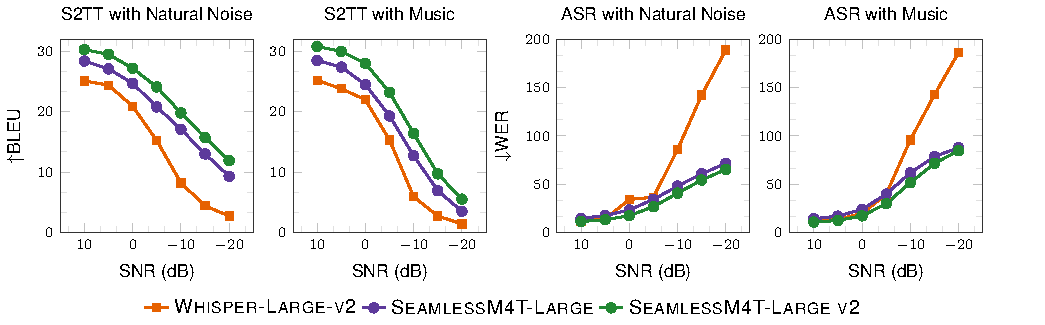
\includegraphics[width=1.1\linewidth]{figures/evaluation/noise_robustness_row_v2.pdf}
    \caption{\textbf{Evaluation results of model robustness against background noise.} We report average test \bleu and test \wer over four languages (three language families) for \xeng~\st and ASR on \fleurs with low-to-high input noise level (high-to-low SNR). Simulated noises are sampled from MUSAN~\citep{snyder2015musan} on the ``noise'' and ``music'' categories. }
    \label{fig:robustness_noise}
\end{figure}

\paragraph{Robustness against background noise.} \Cref{fig:robustness_noise} shows the average test \bleu and test \wer over the four languages for \xeng{} \st and \asr on \fleurs with low-to-high input noise level (high-to-low SNR). Both \bleu-SNR curves for our new model, \mfourtlgtwo are consistently above those for \whisperlarge and \mfourtlg. Similarly, \mfourtlgtwo's \wer-SNR curves are consistently below the ones for \whisperlarge and \mfourtlg. These indicate the superior robustness of \mfourtlgtwo in noisy speaking environments. \mfourtlgtwo outperforms \whisperlarge by an average of 53.2\% and 50.5\% over various noise types and levels for \xeng{} \st and \asr, respectively. It also outperforms our earlier model, \mfourtlg by an average of 14.9\% and 14.5\% for \xeng{} \st and \asr, respectively.




\begin{table}[htb]
    \centering
    \small
    \begin{tabular}{lcccc}
        \toprule
        \multirow{2}{*}{\textbf{Model}} & \multicolumn{2}{c}{\textbf{\fleurs~\xeng~\st}} & \multicolumn{2}{c}{\textbf{\fleurs~\asr}} \\
        \cmidrule(lr){2-3}\cmidrule(lr){4-5}
        & chrF$_{MS}$$\uparrow$ & CoefVar$_{MS}$$\downarrow$ & chrF$_{MS}$$\uparrow$ & CoefVar$_{MS}$$\downarrow$ \\
        \midrule[\heavyrulewidth]
        \whisperlarge & 40.8 & 13.7 & 58.7 & 17.0 \\
        \mfourtlg & 45.3 & 9.1 & 72.5 & 6.4 \\
        \mfourtlgtwo & \textbf{51.6} & \textbf{6.3} & \textbf{79.2} & \textbf{4.0} \\
        \bottomrule
    \end{tabular}
\caption{\textbf{Evaluation results of model robustness against vocal style variations.} We report test average by-group mean chrF (chrF$_{MS}$) and test average by-group coefficient of variation on chrF (CoefVar$_{MS}$) for \xeng~\st and ASR on \fleurs (77 and 78 source languages respectively which have at least 40 content groups).}
\label{tbl:robustness-speaker-variation}
\end{table}

\paragraph{Robustness against vocal style variations.} \Cref{tbl:robustness-speaker-variation} shows the $\textrm{chrF}_{MS}$ and $\textrm{CoefVar}_{MS}$ scores of \mfourtlgtwo, \mfourtlg and \whisperlarge on \fleurs~\xeng~\st and \asr test sets. We see that \mfourtlgtwo outperforms \whisperlarge on $\textrm{CoefVar}_{MS}$ by an average of 66.4\% over \xeng~\st and \asr tasks. Moreover, \mfourtlgtwo outperforms \whisperlarge on chrF$_{MS}$ by an average of 31.5\%. Note that \mfourttwo also outperforms \mfourtlg on both tasks and metrics. These suggest the superior robustness of \mfourtlgtwo when it comes to vocal style variations.


\paragraph{Key findings} Tested for robustness, our system performs better against background noises and vocal style variations in speech-to-text tasks (average improvements of 42\% and 66\%, respectively) compared to \whisperlarge.

\subsection{Human Evaluation}
\label{sec:humaneval}
We present a subset of human evaluation results, focusing on expressivity models for most languages and directions (see \Cref{table:evalsummary} for a summary of available evaluations presented in this section). In a later update, we will present the complete set of human evaluations, including the full set of languages, directions, and models. 

First, we provide an overview of each protocol used in human evaluations, a description of human evaluation benchmark test-set data, followed by analysis and results.

\subsubsection{Human evaluation protocols}
\label{sec:humaneval_protocols}

\begin{table}[!ht]
\centering

\small
\begin{tabular}{cccc}
\toprule
{\bf Protocol} & {\bf Direction} & {\bf Systems} & {\bf Languages} \\
\midrule
PCP & \xeng & 5 & 5 \\
PCP & \engx & - & - \\
\midrule
MOS & \xeng & 5 & 3 \\
MOS & \engx & 5 & 5
\\
\bottomrule
\end{tabular}
\caption{\label{table:evalsummary} Summary of evaluations: languages, models, and protocols used in the current expressivity human evaluations. Note that at the time of writing, human evaluation for PCP had not been completed in the \engx direction.}
\end{table}









\paragraph{MOS.}
\label{sec:mos} 
As in \citet{SeamlessM4TArXiv}, we adopted the Mean Opinion Score (MOS) protocol (a 5-point Likert scale) \cite{p808} to evaluate the speech quality of all models presented in this paper, except for a subset of data in the \xeng direction.\footnote{In particular, for expressivity, we only evaluated MOS on a subsample of $n$=100 items from each dataset in the \xeng direction} The MOS protocol utilized here measures three aspects:

\begin{enumerate}
\item \textbf{Naturalness}: ``how natural is the speech?''
\item \textbf{Sound quality}: ``how good is the sound quality?''
\item \textbf{Speech clarity}: ``how clear is the speech?''
\end{enumerate}

A more detailed protocol explanation can be found in \citet{SeamlessM4TArXiv}. In this work, each item is evaluated by three annotators. No calibration set is evaluated, and we did not source additional annotators upon disagreement, as we did for Cross-Lingual Semantic Textual Similarity (XSTS; \citep{licht2022xsts}, \citep{SeamlessM4TArXiv}).



\paragraph{PCP.}
\label{sec:pcp}
To measure the extent to which expressive characteristics are matched between source- and target-audio, we used a modified version of the Prosodic Consistency Protocol (PCP), previously presented in \cite{huang2023holistic}. In this task, bilingual annotators are asked to listen to both source and target audio and rate similarity along three “expressive” dimensions—\textit{rhythm}, \textit{emotion}, and \textit{overall expressive intent} (abbreviated \textit{OEI} throughout) and one \textit{semantic} dimension, using a 4-pt Likert scale ranging from \textit{1— Completely different} to \textit{4— Completely similar}. Annotators were asked to complete this task while ignoring differences in the speakers' voices. This represents a reduced set of prosodic dimensions (minus \textit{emphasis} and \textit{intonation}) compared to the original protocol presented in \citet{huang2023holistic}. The simplification in expressive aspects, along with refinements in annotator instructions and the inclusion of more diverse language examples, reflects a more cross-linguistic compatible protocol amenable to “distant” language pairs, including English-Mandarin, as evaluated in this work. The entire protocol can be viewed (with format adapted) in \Cref{sec:PCP_protocol_text}.

\paragraph{PCP annotation process.} During annotation, five bilingual annotators\footnote{Annotators must pass language proficiency tests to be included in the study.} examined each source-target audio pair and evaluated the pair's similarity in \textit{semantics}, \textit{emotion}, \textit{rhythm}, and \textit{OEI} using the PCP protocol.  Before annotating, all annotators went through a set of pre-study calibration (practice) examples with score justifications. To expedite evaluation, more than five annotators were used per language pair (up to $n=40$); each evaluated sentence pair was shown to five annotators, assigned randomly. The median score over annotators of the same audio pair was then taken for each evaluation sentence pair; the median is used for robustness. For overall direction scores, we report the mean of this median score across all evaluated items in the dataset generated by a particular system in a language direction.

\subsubsection{Human evaluation test sets}


\label{sec:human_eval_test_sets}
\paragraph{Expressivity benchmark test-sets.} Human evaluations for the Expressivity comparison set (Models 2-5 as described in \Cref{tab:expressive_models}) were conducted on a subset of test partitions (\Cref{tab:expressive_dev_test_data}) selected from mExpresso, mDRAL, and \fleurs test partitions (see \Cref{tab:expressivity-benchmark-sets-descr-stats}). Filtering logic for the benchmark test-set required that all samples be 1 second or longer in duration and contain at least three tokens (or characters when appropriate).

Each domain in the benchmark test set contributes different characteristics of interest. Given these differences, human evaluation protocols were selectively assigned to domains in the benchmark set for which the underlying data contained variations of interest. For example, mExpresso read-speech recordings are acted in distinctive styles, which make use of the PCP protocol appropriate. We evaluated MOS-quality measures across all domains; however, we subsampled in the \xeng direction by domain as we did not expect significant variation between languages translated into English. \Cref{tab:expressivity-benchmark-sets-by-protocol} summarizes the mapping between protocols and benchmark test sets.

\paragraph{mExpresso human evaluation test set.} mExpresso data is described in \Cref{subsec:mexpresso} (along with the collection procedure in \Cref{sec:expressive_data_collection}), however we provide additional details here. Data in this test set is unique among the Expressive evaluation sets as all utterances are pivoted through the original English read-speech collection of \citep{nguyen2023expresso}. That is, semantic content and read styles are matched across all languages for \xeng and \engx directions. To this end, we sampled the mExpresso human evaluation test-set such that samples (in their content and styles) are matched across the languages. The final mExpresso style-set includes ``confused'', ``default'', ``enunciated'', ``happy'', ``sad'',  ``whisper''.

\paragraph{mDRAL human evaluation test set.} mDRAL data is described in \Cref{subsec:mDRAL} (along with the collection procedure in \Cref{sec:expressive_data_collection}), however we provide additional details here. mdRAL data is the only benchmark set in which reference source- and target-speakers are matched. Due to the nature of the collection process (spontaneous conversations occur in one language, then re-enacted by the original bi-lingual speakers in the second language), we sampled our benchmark test set to ensure near-uniform coverage across speakers.

\paragraph{\fleurs human evaluation test set.} Test data was sampled from the test-partition of \fleurs data \citep{conneau2020unsupervised} for each language pair. \citet{SeamlessM4TArXiv} gives a more complete overview of the \fleurs test-set and standard sampling recipes for conducting translation quality evaluation such as XSTS \citep{licht2022xsts}. For the current Expressivity human evaluation, in which we were only interested in evaluating MOS-measures on FLEURs, we sampled uniformly from the test set.

\begin{table}[htp!]
    \centering
    \begin{tabular}{rcc}
        \toprule
         & \begin{tabular}{@{}c@{}} \textbf{PCP} \end{tabular} &  \begin{tabular}{@{}c@{}} \textbf{MOS} \end{tabular}\\
        \midrule
        mExpresso & \greencheck &  \greencheck \\
        mDRAL & \greencheck &  \greencheck\\
        \fleurs & \redxmark &  \greencheck\\
        \bottomrule
    \end{tabular}
    \caption{Protocol use by Human Evaluation benchmark test-set domain.}
    \label{tab:expressivity-benchmark-sets-by-protocol}
\end{table}

\begin{table}[htbp!]
    \small
    \centering
    \begin{tabular}{lrrr}
        \toprule
         & \textbf{mExpresso} & \textbf{mDRAL} & \textbf{\fleurs} \\ \midrule
        Sample \#              & 4818 &  2020  & 1500 \\
        Hours                  & 6.24 & 2.07   & 4.47 \\
        Total \# Speakers      & 9    & 55     & - \\
        Total \# Male Speakers & 4    & 19     & - \\
         \hline
    \end{tabular}
    \caption{Descriptive statistics of the human evaluation benchmark test-set aggregating over all language directions. Note that we do not have speaker information for \fleurs so these rows are left empty.}
    \label{tab:expressivity-benchmark-sets-descr-stats}
\end{table}

\subsubsection{Analysis and results}
\label{sec:human_eval_analysis_results}
We present an analysis of available human evaluation data focusing on the language pair by protocol combinations with adequate samples. Please note the use of model identifiers, which refer to model naming conventions described in \Cref{tab:expressive_models}. Throughout, we report bootstrap re-sampled mean and standard error estimates, re-sampling $n_b=500$ times at the item level. At the time of writing, we had sufficient sample to report results on a subset of PCP \xeng directions (excluding cmn and fra) and no results in the \engx direction. We report results for all MOS directions. Subsequent updates will include data and analysis for the remaining language directions and protocols. Note that unless stated otherwise, in both tables and written text we standardly report estimated mean values with standard errors included in parentheses.


\paragraph{A note on baseline model (\mfourttwo) used in Expressivity Human Evaluation.}
\label{sec:human_eval_expr_baseline_model_discussion}

For transparency, we note that there is a minor difference in the baseline systems (Model 2, \mfourttwo) used to report Human Evaluation results and used to report automatic evaluation results (\Cref{subsec:express_exp}). The discrepancy is based on how the two models' unit-level duration information is produced during inference. In particular, the model used in the automatic results section uses a frame-level sequence of acoustic units, which are then used by a unit vocoder to produce the waveform. In contrast, the human evaluation baseline model relied on a unit vocoder to generate frame-level duration using the reduced sequence of acoustic tokens. That mismatch has shown only a slight change in the automatic scores as described in \Cref{app:expressive}. Given the minimal changes to automatic scores, we do not believe this discrepancy impacts conclusions related to the comparison of the baseline and Expressivity models.

\paragraph{Key findings}
\begin{itemize}
    \item \ptv. Comparisons between Model 2 (\mfourttwo) and Model 3 (\mfourttwo+\ptv) serve as an ablation of the \ptv module. We see consistent improvement with the inclusion of \ptv with higher scores for Model 3 across all PCP expressive dimensions, but with declines in some MOS subscores.
    
    On expressivity dimensions, aggregating across language and datasets, we see nominal improvements for ``rhythm'' ($\delta$=0.30; 3.03 (0.14) vs 2.73 (0.14)), ``emotion'' ($\delta$=0.60; 3.18 (0.13) vs 2.58 (0.14)), and ``OEI'' ($\delta$=0.39; 3.03 (0.11) vs 2.64 (0.11)) across all \xeng directions (see rows 4 and 5 of \Cref{tab:express_human_eval_pcp_direction_agg} for within-domain results). While variation between languages exists, \ptv has higher PCP subscores compared to \mfourttwo for all languages (see \Cref{tab:pcp_human_evaluation_full_table}). 
    
    On MOS dimensions, aggregating over languages by system we observe that the addition of the \ptv module results in lower MOS subscores for ``clarity of speech'' ($\delta$=-0.49; 4.09 (0.08) vs 4.58 (0.06)) and ``sound quality'' ($\delta$=-0.79; 3.64 (0.08) vs 4.42 (0.07)), but remains at parity for ``naturalness'' ($\delta$=0.03; 4.01 (0.09) vs 3.97 (0.09)) compared to the \mfourttwo model without the \ptv module (see \Cref{tab:express_human_eval_mos_direction_agg_mean_vals} for within-domain results). 

    \item \mfourttwo+\ptv vs \seamlessexpressive. Comparisons between Model 3 (\mfourttwo+\ptv) and Model 5 (\seamlessexpressive) serve as an ablation of the \prosodyunitytwo component, which controls the speech rate and pauses. We see consistent improvement across all PCP expressive dimensions, but with some declines in MOS ``naturalness'' subscores.
    
    On expressivity dimensions, aggregating across language and datasets, we see improvements for ``rhythm'' ($\delta$=0.58; 3.60 (0.07) vs 3.03 (0.14)), ``emotion'' ($\delta$=0.41; 3.60 (0.08) vs 3.18 (0.13)), and ``OEI'' ($\delta$=0.44; 3.47 (0.09) vs 3.03 (0.11)). Note that in the case of mExpresso data, in which different speakers enact source- and target-pairs, Model 5 (and Model 4 for that matter) exceeds Human Reference on PCP expressive dimensions. While Model 5 PCP scores are also high for mDRAL, they do not reach the level of Human Reference (see \Cref{tab:express_human_eval_pcp_direction_agg}).

    On MOS dimensions, aggregating across language and datasets, we see that Model 5 has lower ``naturalness'' ratings, ($\delta$=-0.38; 3.62 (0.11) vs 4.01 (0.09)), but is at parity for ``sound quality'' and ``clarity of speech'' ($\delta$=-0.03; 3.60 (0.08) vs 3.64 (0.08)) subscores. Of the current comparison set, Model 5 performs worst overall on ``naturalness'' and ``sound quality'' ratings.
    
    \item \seamlessexpressive vs. \prosodyunitytwo+\unitvb. Comparisons between Model 5 (\seamlessexpressive) and Model 4 (\prosodyunitytwo+\unitvb) serve as an ablation of the speech generation module. Results indicate that the use of \unitvb can further improve on MOS subscores, including ``clarity of speech" ($\delta$=0.26; 4.41 (0.06) vs 4.14 (0.07)) and ``sound quality'' ($\delta$=0.55; 4.15 (0.07) vs 3.60 (0.08)), while it does not improve on the aspects of expressivity preservation.
\end{itemize}


\begin{table}[htbp!]
\small
\centering
\begin{tabular}{ccccccc}
\toprule
  & \multicolumn{3}{c}{\textbf{mDRAL}} & \multicolumn{3}{c}{\textbf{mExpresso}}\\ 
\cmidrule(rr){2-4}\cmidrule(rr){5-7}
\textbf{ID} & OEI & Emotion & Rhythm & OEI & Emotion & Rhythm \\ 
\midrule

{\xeng}\\
\midrule
Reference  & 3.71 (0.08) & 3.82 (0.09) & 3.82 (0.08) & 3.33 (0.07) & 3.38 (0.07) & 3.54 (0.07) \\
5          & 3.48 (0.11) & 3.48 (0.09) & 3.65 (0.08) & 3.46 (0.06) & 3.56 (0.06) & 3.56 (0.06) \\ 
4          & 3.42 (0.12) & 3.42 (0.10) & 3.59 (0.11) & 3.35 (0.06) & 3.56 (0.07) & 3.55 (0.07) \\
3          & 3.18 (0.14) & 3.27 (0.16) & 3.20 (0.17) & 2.89 (0.07) & 3.09 (0.09) & 2.85 (0.11) \\
2          & 2.79 (0.16) & 2.79 (0.19) & 2.90 (0.19) & 2.50 (0.07) & 2.44 (0.09) & 2.56 (0.10) \\
\midrule 
\bottomrule
\end{tabular}
\caption{Human Evaluation results for PCP expressive dimensions (scale is 1-4). Cells contain mean values (std. errors) aggregated over language-pair results. Note that at the time of writing, human annotation for PCP \engx direction was not yet available for analysis. See \Cref{tab:pcp_human_evaluation_full_table} for aggregate scores on the language direction and dataset level.} \label{tab:express_human_eval_pcp_direction_agg}
\end{table}

\begin{table}[htbp!]
\centering
\small
\begin{tabular}{cccccccccc}
\toprule
 & \multicolumn{3}{c}{\textbf{\fleurs}} & \multicolumn{3}{c}{\textbf{mDRAL}}  & \multicolumn{3}{c}{\textbf{mExpresso}}\\ 
\cmidrule(rr){2-4}\cmidrule(rr){5-7}\cmidrule(rr){8-10}
\textbf{ID} & Clar. & Nat. & Qual. & Clar. & Nat. & Qual. & Clar. & Nat. & Qual.\\ 
\midrule
\xeng \\
\midrule
Reference   & 4.68 & 4.79 & 3.65 & 4.48 & 4.67 & 4.58 & 4.95 & 4.52 & 4.97 \\
5           & 4.69 & 3.85 & 4.03 & 4.63 & 3.70 & 4.21 & 4.71 & 3.87 & 4.23 \\
4           & 4.79 & 3.82 & 4.63 & 4.82 & 3.75 & 4.58 & 4.84 & 4.02 & 4.61 \\
3           & 4.63 & 4.27 & 3.99 & 4.59 & 4.19 & 4.09 & 4.59 & 4.16 & 4.25 \\
2           & 4.76 & 4.32 & 4.24 & 4.85 & 4.32 & 4.52 & 4.77 & 4.27 & 4.47 \\

\midrule 
\midrule
\engx \\%& \multicolumn{3}{c|}{\fleurs} & \multicolumn{3}{c|}{mDral} & \multicolumn{3}{c|}{mExpresso} \\ 
\midrule
Reference   & 4.36 & 4.52 & 4.00 & 4.35 & 4.61 & 4.23 & 4.40 & 4.27 & 4.24 \\
5           & 2.98 & 3.48 & 2.34 & 4.14 & 3.68 & 3.55 & 4.03 & 3.28 & 3.58 \\
4           & 3.56 & 3.67 & 2.97 & 4.37 & 3.82 & 4.06 & 4.29 & 3.37 & 4.32 \\
3           & 2.94 & 3.65 & 2.36 & 4.06 & 4.00 & 3.64 & 4.02 & 3.88 & 3.77 \\
2           & 4.34 & 3.71 & 4.39 & 4.46 & 3.70 & 4.43 & 4.42 & 3.73 & 4.49 \\
\bottomrule
\end{tabular}
\caption{Human Evaluation results for MOS dimensions—mean estimates (scale is 1-5). Cells contain mean values aggregated over language-pair results. Please see \Cref{tab:express_human_eval_mos_direction_agg_se_vals} for the corresponding std. error estimates, \Cref{tab:mos_human_evaluation_full_table_mu} for aggregate scores at the language direction by dataset level and \Cref{tab:mos_human_evaluation_full_table_se} for associated standard errors of aggregated scores at the language direction by dataset level.}\label{tab:express_human_eval_mos_direction_agg_mean_vals}
\end{table}

\begin{table}[htbp!]
\centering
\small
\begin{tabular}{cccccccccc}
\toprule
 & \multicolumn{3}{c}{\textbf{\fleurs}} & \multicolumn{3}{c}{\textbf{mDRAL}}  & \multicolumn{3}{c}{\textbf{mExpresso}}\\ 
\cmidrule(rr){2-4}\cmidrule(rr){5-7}\cmidrule(rr){8-10}
\textbf{ID} & Clar. & Nat. & Qual. & Clar. & Nat. & Qual. & Clar. & Nat. & Qual.\\ 
\midrule
\xeng \\
\midrule
Reference   & 0.10 & 0.07 & 0.14 & 0.10 & 0.10 & 0.08 & 0.02 & 0.07 & 0.01 \\
5           & 0.08 & 0.13 & 0.11 & 0.09 & 0.20 & 0.13 & 0.08 & 0.13 & 0.09 \\
4           & 0.06 & 0.13 & 0.07 & 0.06 & 0.16 & 0.10 & 0.04 & 0.12 & 0.07 \\
3           & 0.08 & 0.10 & 0.10 & 0.12 & 0.17 & 0.14 & 0.10 & 0.12 & 0.10 \\
2           & 0.07 & 0.11 & 0.08 & 0.06 & 0.14 & 0.09 & 0.07 & 0.12 & 0.10 \\
\midrule
\midrule
\engx \\ %
\midrule
\midrule
Reference   & 0.06 & 0.06 & 0.07 & 0.06 & 0.05 & 0.06 & 0.03 & 0.03 & 0.03 \\
5           & 0.10 & 0.09 & 0.09 & 0.06 & 0.07 & 0.06 & 0.03 & 0.04 & 0.03 \\
4           & 0.09 & 0.08 & 0.10 & 0.06 & 0.08 & 0.06 & 0.03 & 0.04 & 0.03 \\
3           & 0.10 & 0.09 & 0.09 & 0.07 & 0.07 & 0.06 & 0.04 & 0.04 & 0.03 \\
2           & 0.07 & 0.08 & 0.06 & 0.06 & 0.08 & 0.05 & 0.03 & 0.04 & 0.03 \\
\bottomrule
\end{tabular}
\caption{Human Evaluation results for MOS dimensions - standard errors. Cells contain standard errors aggregated over language-pair results.}
\label{tab:express_human_eval_mos_direction_agg_se_vals}
\end{table}

\subsubsection{Understanding MOS-quality measures for expressive models}
\label{sec:p2v_sensitivity}
Results as discussed in \Cref{sec:human_eval_analysis_results} indicate a somewhat curious finding—the inclusion of expressivity-preserving modules such as \ptv and \prosodyunitytwo (in particular Models 3 and 5) lead to substantial improvements on expressivity-preservation measures such as ``Rhythm'', ``Emotion'' and ``OEI.'' However, these improvements appear to come at a cost of lower ``Sound Quality'' and ``Clarity of Speech'', as measured by the MOS protocol (\Cref{tab:express_human_eval_pcp_direction_agg}). We explore the hypothesis that sensitivity to acoustic features (of speaker vocal style and recordings), which allows the models to preserve high-level expressive characteristics, may also make the models sensitive to unwanted artifacts located in source audio. To do so, we examine four acoustic measures of speech that are often used in studies of speech pathology and audio quality, namely the signal-to-noise ratio (SNR), harmonics-to-noise ratio (HNR), shimmer, and jitter.

\paragraph{Measuring noise-like characteristics in speech.} SNR, HNR, jitter, and shimmer describe different aspects of speech's noise-like characteristics. SNR measures the energy ratio between speech and non-speech signal of an audio waveform. HNR measures the energy ratio between periodic and aperiodic components of the speech signal. Higher values of SNR and HNR can generally be interpreted as less background noise (or cleaner audio) and less rough or hoarse-sounding speech (or a more stable speech signal), respectively. Jitter and shimmer measure pathological instability characteristics of vocalization. Specifically, jitter quantifies the instability of vocal fold vibration (pitch). Shimmer quantifies the instability of the amplitude of the speech waveform. High jitter and high shimmer values are often interpreted as the speech sounding as if it is trembling and coarse sounding, respectively.\footnote{Jitter and Shimmer were computed using the openSMILE audio feature extraction toolkit \citep{opensmile} (using the eGeMAPSv02 feature set). HNR was computed using PRAAT implementation parselmouth \citep{parselmouth}. SNR was computed using an internal library.}

\paragraph{A comparison of the acoustic correlates of expressivity and noise.} We compute utterance-level SNR, HNR, jitter, and shimmer for both source and target audio\footnote{For this analysis, we restrict ourselves to pairs for which both source- and target-audio had MOS ratings (reducing the total sample to $n=19233$ items).} for our Expressivity comparison set (\Cref{fig:snr.hnr.shimmer.jitter-pointwise-correlations}). We analyze the data in three ways. First, we examine the degree to which each of our systems preserves these acoustic characteristics by examining the correlation between measures for input source and output target speech. Examining the correlation values gives us an indication of how well these characteristics are preserved by each model. Second, we compute the average difference between source and target values to measure the degree to which the systems either reduce or amplify these characteristics. Third, we examine the overall relationship between these acoustic features and MOS ratings for target outputs.

As shown in \Cref{fig:snr.hnr.shimmer.jitter_correlations}, the correlation results indicate that all expressivity-preserving models preserve SNR, HNR, shimmer, and jitter from source audio to some extent, and significantly over what we see with \mfourttwo (for which target outputs are essentially independent of source inputs for these acoustic characteristics). In particular, HNR is preserved to the largest degree in models that make use of the \ptv module (Models 3 and 5). 

\begin{figure}[t]
    \centering
    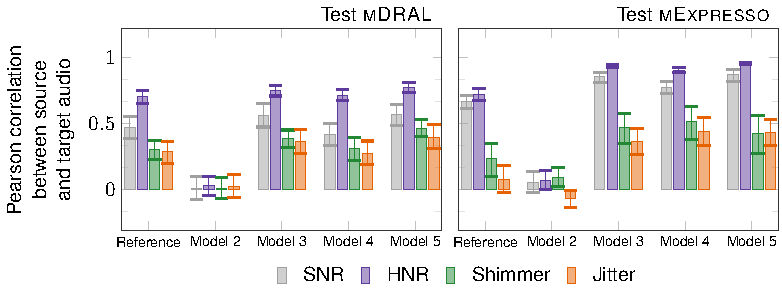
\includegraphics[width=\linewidth]{figures/evaluation/snr_hnr_shimmer_jitter_correlations.pdf}
    \caption{Correlation between source- and target-measures of ``SNR'', ``HNR'', ``shimmer'', and ``jitter''. Mean correlation values and confidence intervals estimated via bootstrap re-sampling with $n_b=500$.}
    \label{fig:snr.hnr.shimmer.jitter_correlations}
\end{figure}

In addition, we examine the degree to which expressivity-preserving models reduce or amplify these acoustic characteristics. Interestingly, all models perform noise reduction to some degree, as measured by SNR. However, this effect is most pronounced in Model 2 (\mfourttwo) and reduced in both Models 3 and 5 (\mfourttwo+\ptv and \seamlessexpressive) (gray bars of \Cref{fig:snr.hnr.shimmer.jitter_diffs}). Of particular import, the negative components of HNR, which are realized in more hoarse or breathy sounding speech, is actually \textit{increased} (lower HNR values) in Models 3 and 5 (purple bars of \Cref{fig:snr.hnr.shimmer.jitter_diffs}).

\begin{figure}[t]
    \centering
    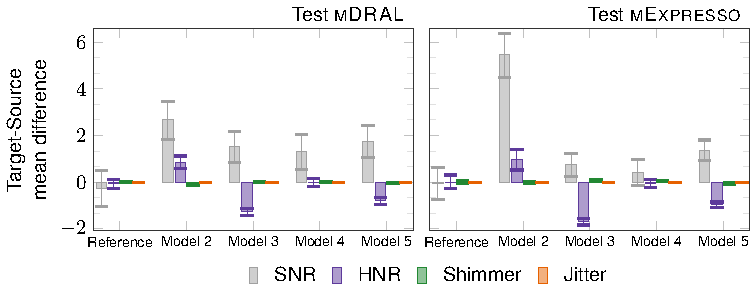
\includegraphics[width=\linewidth]{figures/evaluation/snr_hnr_shimmer_jitter_diffs.pdf}
    \caption{The average difference between paired target and source audios for ``SNR'', ``HNR'', ``shimmer'', and ``jitter'' values. Lower values for HNR indicate more perceived hoarseness in speaker speech, while higher HNR indicates less perceived hoarseness. Mean estimates and 95\% CIs computed from $n_b=500$ bootstrap resampling.}
    \label{fig:snr.hnr.shimmer.jitter_diffs}
\end{figure}

Up to this point, we have shown that the expressivity models uniquely preserve features of source audio in target outputs, and in the case of Models 3 and 5, aspects such as HNR are actually amplified. We now examine the relation between noise-related features (SNR, HNR, shimmer, and jitter) on MOS ratings across all model-based outputs. To do so, we extract item-level noise features and compute Spearman's Rank correlation with MOS-ratings across the three dimensions ``Clarity of Speech'', ``Sound Quality,'' and ``Naturalness'' (\Cref{fig:snr.hnr.shimmer.jitter-pointwise-correlations}). 

Results (\Cref{fig:snr.hnr.shimmer.jitter-relation-to-mos}) indicate that HNR and SNR have a non-zero (positive) association with ``Clarity of Speech'' ratings while jitter and shimmer appear to have little relation. By contrast, we see that both shimmer and jitter have a substantial positive association with ``Naturalness''—presumably non-pathological amounts of these characteristics are seen as more human-like. Also, we see that HNR has a substantial negative correlation with ``Naturalness,'' meaning that as HNR increases, ``Naturalness'' actually declines. This is a somewhat curious effect, but it may be similar to the finding for shimmer and jitter such that a small amount of breathiness or roughness may be seen as more natural, so long as that level is not pathological. Finally, we see that both HNR and SNR have a substantial positive correlation with ``Sound Quality'' such that higher HNR and SNR values result in higher sound quality ratings. To a small degree, both shimmer and jitter display the opposite association.

This analysis, in the aggregate, provides converging evidence that in some cases (particularly Models 3 and 5), sensitivity to the acoustic correlates of expressivity may also lead to sensitivity to noise-related acoustic features (unless explicitly mitigated), leading to lower ``Sound Quality'' and ``Clarity of Speech'' ratings. These findings are largely consistent with the architecture and training recipes for the current model set. For example, in the case of Model 2 (\mfourttwo), the speech-to-unit translation model is trained on a large amount of pseudo-labeled data with target units generated from a T2U model, and the unit vocoder is trained on a distribution of clean speech without any notion of the noisiness of the source speech during inference. By contrast, during training, the \ptv module (Models 3 and 5) uses reference audio to condition the Mel-filterbank feature distribution it models. During training, it inevitably associates noise patterns between the reference input and the target audio in the Mel-filterbank feature space (where noise is well presented).


\begin{figure}[t]
    \centering
    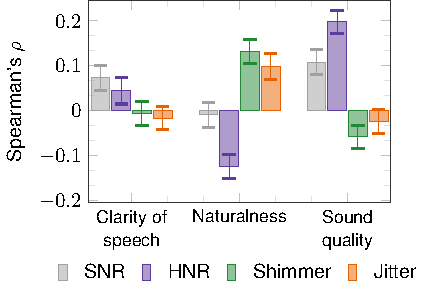
\includegraphics[width=.6\linewidth]{figures/evaluation/snr_hnr_shimmer_jitter_relation_to_mos.pdf}
    \caption{Relation of noise-related features (shimmer, jitter, hnr, snr) and MOS ratings (\textit{Clarity of Speech}, \textit{Naturalness}, and \textit{Sound Quality}. Mean estimates and CIs are computed from bootstrap re-sampling taking $n_b=500$ bootstrap re-samples.}
    \label{fig:snr.hnr.shimmer.jitter-relation-to-mos}
\end{figure}





\subsubsection{Correlation between automatic metrics and human evaluation}
\label{sec:human_eval_correlation_analysis}
We considered the relationship between automatically-derived expressive quality measures (as described in \Cref{sec:expressivity_metrics}) and our Human Evaluation measures (as described in \Cref{sec:humaneval_protocols}).\footnote{Note this analysis is similar in spirit to the analysis presented in \Cref{sec:comparator}.} We examined Spearman rank correlation coefficients for aggregate scores at the level of language-pair, dataset, and system triples. Aggregation at this level makes metrics directly comparable as rhythm-related measures (as described in \Cref{sec:expressivity_metrics}) are only computed at the corpus level and typically aggregated by language-pair, dataset, and system. 

Results suggest that nearly all expressive (or non-semantic) related metrics\footnote{PCP: ``rhythm'', ``emotion'' and ``overall expressive intent''; Automatic: ``AutoPCP'', ``Speaker-sim'', ``Speech-rate'', ``Speech-rate + Pausing'', ``Pausing''} are strongly associated with each-other as measured by the Spearman rank correlation coefficient. By contrast, the association is greatly reduced between expressive- and semantic-related measures\footnote{PCP: ``semantics''; Automatic: \asrbleu and \bleu}, which is expected. All pairwise correlations can be viewed in \Cref{fig:metrics_spearman_matrix}.

Of particular interest is the strong correlation ($\rho=0.796$) between ``AutoPCP'' and the PCP's ``Overall Expressive Intent'' (OEI) dimension (\Cref{fig:eval_metrics_corr}), as well as the correlation between both speech-rate and pausing and PCP's rhythm dimension ($\rho=0.771$ and $\rho=0.811$, respectively). Strong associations between these metrics provide an important sanity check of the validity of both types of measures. The fact that nearly all expressivity-related measures show strong association is not a surprise--while the PCP elicits ratings independently, expressive characteristics such as \textit{emotion}, \textit{rhythm}, and \textit{overall expressive intent} naturally co-vary.\footnote{As a toy example, consider angry or agitated speech--as a listener, the inference that the speaker is ``angry'' is likely in part a function of speech-rate (such that in many languages and cultures faster speech is seen as angrier).}

\begin{figure}[t]
    \centering
    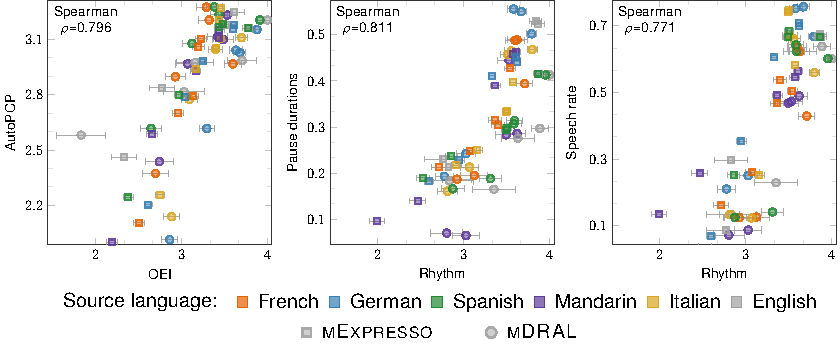
\includegraphics[width=1\linewidth]{figures/evaluation/eval_metrics_corr.pdf}
    \caption{Human Evaluation (PCP) OEI and Rhythm correlations to AutoPCP, Pause durations, and Speech rate automatic metrics. (Automatic metrics displayed on each facet's vertical axis and Human Evaluation (PCP) metrics on horizontal axis.) Correlations are Spearman Rank Correlation Coefficients computed on language-pair, data, and system aggregations. Error bars represent analytic-based 95\% CIs for human ratings.}
    \label{fig:eval_metrics_corr}
\end{figure}







